\documentclass[11pt]{book}
\usepackage{gvv-book}
\usepackage{gvv}
\usepackage[sectionbib,authoryear]{natbib}
\setcounter{secnumdepth}{3}
\setcounter{tocdepth}{2}
\makeindex
\begin{document}
\frontmatter
\tableofcontents
\setcounter{page}{1}
\mainmatter
\chapter{Triangle}
Consider a triangle with vertices
\begin{align}
\label{eq:tri-pts}
\vec{A}=\myvec{1 \\ 3},\,
\vec{B}=\myvec{-3\\0},\,
	\vec{c}=\myvec{0\\4},\,
\end{align}

\section{Vectors}


\begin{enumerate}[label=\thesection.\arabic*.,ref=\thesection.\theenumi]
\numberwithin{equation}{enumi}

\item The direction vector of $AB$ is defined as
		\begin{align}
			\vec{B}-
			\vec{A}
		\end{align}


Question1.1.1 :Find the Direction Vectors of $AB$,$BC$ and $CA$.\\
\solution

\begin{enumerate} 
\item  The Direction vector of $AB$ is \begin{align} &
\vec{B} - \vec{A} = \myvec{-3 \\ 0}-\myvec{1 \\ 3}=\myvec{ -3 - (1)\\ 0 - (3) } = \myvec{ -4\\ -3 }
 \end{align}
 
\item The Direction vector of $BC$ \begin{align}&
\vec{C} - \vec{B} = \myvec{0 \\ 4}-\myvec{-3 \\ 0}=\myvec{ 0 - (-3)\\ 4 - (0) } = \myvec{ 3\\ 4 }
  \end{align}
  
  \item  The Direction vector of $CA$  \begin{align} &
  \vec{A} - \vec{C} = \myvec{1 \\ 3}-\myvec{0 \\ 4}=\myvec{ 1 - (0)\\ 3 - (4) } = \myvec{ 1\\ -1 }
  \end{align}
 \end{enumerate}

\item The length of side $BC$ is 
		\begin{align}
			\norm{\vec{B}-\vec{A}} \triangleq \sqrt{\brak{\vec{B}-\vec{A}}^{\top}{\vec{B}-\vec{A}}}
		\end{align}
		where
		\begin{align}
			\vec{A}^{\top}\triangleq\myvec{1 & 3}
		\end{align}
Question 1.1.2 : Find the length of side AB, BC, CA.\\
\solution
 
 
 (a) 
 Solving for AB
 
 %\vec{A} - \vec{B} & = \myvec{4 \\ 3} \\
  \begin{align}
 \norm{\vec{A}-\vec{B}}\ &=  \sqrt{\brak{\vec{A}-\vec{B}}^{\top}\brak{\vec{A}-\vec{B}}} \\
 \vec{A}-\vec{B} &= \myvec{1 \\ 3} - \myvec{-3 \\ 0} = \myvec{4 \\ 3} \\
 \brak{\vec{A}-\vec{B}}^{\top} &= {\myvec{4 \\ 3}}^{\top} = \myvec{4 \ 3} \\
\brak{\vec{A}-\vec{B}}^{\top}\brak{\vec{A}-\vec{B}} &= \myvec{4 \ -3} \myvec{4 \\ 3} = 16+9 = 25 \\  
 \implies \norm{\vec{A}-\vec{B}}\ &=\sqrt{\brak{\vec{A}-\vec{B}}^{\top}\brak{\vec{A}-\vec{B}}} = \sqrt{25} = 5
\end{align}
(b)
Solving for BC 
 
 %\vec{B} - \vec{C} & = \myvec{-3 \\ -4} \\
  \begin{align}
 \norm{\vec{B}-\vec{C}}\ &=  \sqrt{\brak{\vec{B}-\vec{C}}^{\top}\brak{\vec{B}-\vec{C}}} \\
 \vec{B}-\vec{C} &= \myvec{-3 \\ 0} - \myvec{0 \\ 4} = \myvec{-3 \\ -4} \\
 \brak{\vec{B}-\vec{C}}^{\top} &= {\myvec{-3 \\ -4}}^{\top} = \myvec{-3 \ -4} \\
\brak{\vec{B}-\vec{C}}^{\top}\brak{\vec{B}-\vec{C}} &= \myvec{-3 \ -4} \myvec{-3 \\ -4} = 9+16 = 25 \\  
 \implies \norm{\vec{B}-\vec{C}}\ &=\sqrt{\brak{\vec{B}-\vec{C}}^{\top}\brak{\vec{B}-\vec{C}}} = \sqrt{25}	= 5 
\end{align}
(c)
Solving for CA

 %\vec{C}-\vec{A}  &=\myvec{-1 \\ 1} \\
  \begin{align}
 \norm{\vec{C}-\vec{A}}\ &=  \sqrt{\brak{\vec{C}-\vec{A}}^{\top}\brak{\vec{C}-\vec{A}}} \\
 \vec{C}-\vec{A} &= \myvec{0 \\ 4} - \myvec{1 \\ 3} = \myvec{ -1\\ 1} \\
 \brak{\vec{C}-\vec{A}}^{\top} &= {\myvec{-1 \\ 1}}^{\top} = \myvec{-1 \ 1} \\
\brak{\vec{C}-\vec{A}}^{\top}\brak{\vec{C}-\vec{A}} &= \myvec{-1 \ 1} \myvec{-1 \\ 1} = 1+1 = 2 \\  
 \implies \norm{\vec{C}-\vec{A}}\ &=\sqrt{\brak{\vec{C}-\vec{A}}^{\top}\brak{\vec{C}-\vec{A}}} = \sqrt{2}	 
\end{align}



\item   Points $\vec{A}, \vec{B}, \vec{C}$ are defined to be collinear if 
		\begin{align}
			\rank{\myvec{1 & 1 & 1 \\ \vec{A}& \vec{B}&\vec{C}}} = 2
		\end{align}
Are the given points in
			\eqref{eq:tri-pts}
collinear?\\
Question 1.1.3 : Check the collinearity of $\vec{A},\vec{B},\vec{C}$ \\ 
\solution 
Given that,
\begin{align}
    \vec{A} = \myvec{1\\3}
    \quad
    \vec{B} &= \myvec{-3\\0}
    \quad
    \vec{C} = \myvec{0\\4}
\end{align}
Given that $\vec{A},\vec{B},\vec{C}$ are collinear if
\begin{align}
    \text{rank}\myvec{
    1 & 1 & 1\\
    \vec{A} & \vec{B} & \vec{C} \\
    } &< 3 
    \label{eq:1.1.3,2}
\end{align} 
Let
\begin{align}
    \vec{R}&=\myvec{
    1 & 1 & 1
    \\
    1 & -3 & 0
    \\
    3 & 0 & 4
    } 
\end{align} 
The matrix $\vec{R}$ can be row reduced as follows,
\begin{align}
    \label{eq:matthrowoperations}
    \myvec{
    1 & 1 & 1
    \\
    1 & -3 & 0
    \\
    3 & 0 & 4
    }
     \xleftrightarrow[]{R_3 \leftarrow R_3+5R_1}
    \myvec{
    1 & 1 & 1
    \\
    1 & -3 & 0
    \\
    4 & -3 & 4 
    }
    \\
     \xleftrightarrow[]{R_2\leftarrow R_2+3R_1}
    \myvec{
    1 & 1 & 1
    \\
    0 & 4 & 1
    \\
    4 & -3 & 4 
    }
\end{align}
There are no zero rows. So,
\begin{align}
    \text{rank}\myvec{
    1 & 1 & 1\\
    \vec{A} & \vec{B} & \vec{C} \\
    } &= 3 
\end{align}  
Hence, from \eqref{eq:1.1.3,2} the points $\vec{A},\vec{B},\vec{C}$ are not collinear. 

From Fig. \ref{fig1:Triangle}, We can see that $\vec{A},\vec{B},\vec{C}$ are not collinear .
\begin{figure}[H]
\centering
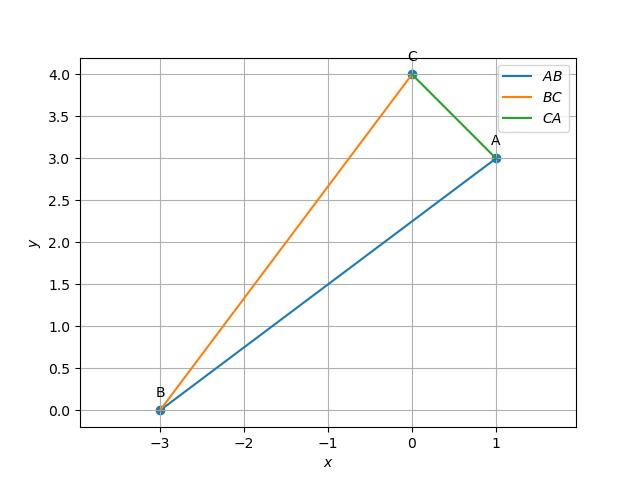
\includegraphics[width=\columnwidth]{/sdcard/hima/geometry/figs/vect.jpg}
\caption{$\vec{A},\vec{B},\vec{C}$ plot}
\label{fig1:Triangle}
\end{figure}



\item The parameteric form of the equation  of $AB$ is 
		\begin{align}
			\vec{x}=\vec{A}+k\vec{m}
		\end{align}
		where
		\begin{align}
\vec{m}=\vec{B}-\vec{A}
		\end{align}
is the direction vector of $AB$.\\
Question 1.1.4 :Find the parametric equation of $AB$,$BC$,$CA$.\\
\solution
The parametric equation for AB is given by
\begin{align}
\vec{x} &= \vec{A} + k\vec{m}\\
\text{where, } \vec{m} &= \vec{B} -\vec{A}\\
&= \myvec{-3 \\ 0} -\myvec{1\\ 3}\\
&= \myvec{-4 \\-3}
\end{align}
Hence we get,
\begin{align}
AB: \vec{x} = &\myvec{1\\3} + k \myvec{-4\\-3}
\end{align}
Similarly, 
\begin{align}
BC: \vec{x} = &\myvec{-3\\0} + k \myvec{3\\4}\\
CA: \vec{x} = &\myvec{0\\4} + k \myvec{1\\-1}
\end{align}


\item The normal form of the equation of $AB$  is 
		\begin{align}
			\vec{n}^{\top}\brak{	\vec{x}-\vec{A}} = 0
		\end{align}
		where 
		\begin{align}
			\vec{n}^{\top}\vec{m}&=\vec{n}^{\top}\brak{\vec{B}-\vec{A}} = 0
			\\
			\text{or, } \vec{n}&=\myvec{0 & 1 \\ -1 & 0} \vec{m}
		\end{align}
  \begin{align}
\vec{n}^{\top}\myvec{\vec{x}-\vec{A}}=0
\end{align}
where
\begin{align}
\vec{n}^{\top}\vec{m}&=\vec{n}^{\top}\myvec{\vec{B}-\vec{A}}=0
\end{align}	
or,\begin{align}
\vec{n}&=\myvec{0 &1 \\-1 & 0}\vec{m}
\end{align}
Question 1.1.5:Find the normal form of the equations of $AB, BC$ and $CA$.\\
\solution:
       The normal equation for the side $AB$ is
\begin{align}
\vec{n}^{\top}\myvec{\vec{x}-\vec{A}}&=0\\
\implies
\vec{n}^{\top}\vec{x}&=\vec{n}^{\top}\vec{A}
\end{align}
Now our task is to find the $\vec{n}$ so that we can find $\vec{n}^{\top}$.
As given in the question 
\begin{align}
  \vec{n} &= \myvec{0 & 1\\
  -1 & 0}\vec{m}
\end{align}
Here $\vec{m} = \vec{B}- \vec{A}$ for side $\vec{AB}$
\begin{align}
\implies
\vec{m}&=\myvec{-3\\0} - \myvec{1\\3}\\
&=\myvec{-4\\-3}
\end{align}
Now as we have obtained vector $\vec{m}$.
we can use this to obtain vector $\vec{n}$
\begin{align}
\vec{n} &= \myvec{0 & 1\\
  -1 & 0}\myvec{-4\\-3}
 = \myvec{-3\\4}
\end{align}
The transpose of $\vec{n}$ is
\begin{align}
  \vec{n}^{\top}&=\myvec{-3 & 4}
\end{align}
Hence the normal equation of side $AB$ is 
\begin{align}
    \myvec{-3 & 4}\vec{x}&=\myvec{-3 & 4}\myvec{1\\3}\\
    \implies
    \myvec{-3 & 4}\vec{x}&= 9
\end{align}
\begin{figure}[H]
	\centering
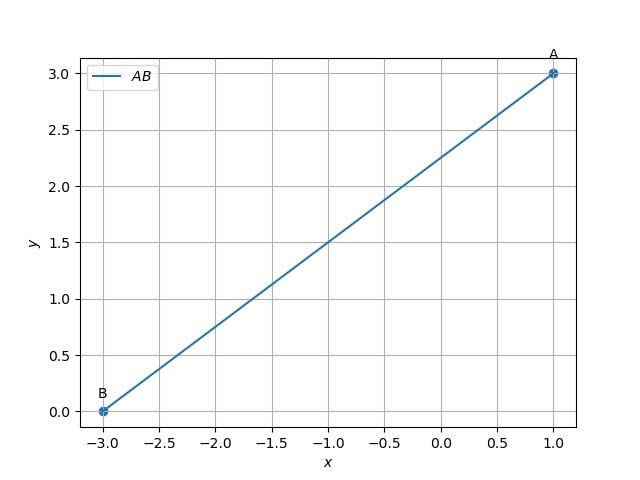
\includegraphics [width=\columnwidth] {/sdcard/hima/geometry/figs/nobe.jpg}
\caption{ The line $\vec{AB}$ plotted using python}
\label{fig: lineab}
\end{figure}


       The normal equation for the side $BC$ is
\begin{align}
\vec{n}^{\top}\myvec{\vec{x}-\vec{B}}&=0\\
\implies
\vec{n}^{\top}\vec{x}&=\vec{n}^{\top}\vec{B}
\end{align}
Now our task is to find the $\vec{n}$ so that we can find $\vec{n}^{\top}$.
As given in the question 
\begin{align}
  \vec{n} &= \myvec{0 & 1\\
  -1 & 0}\vec{m}
\end{align}
Here $\vec{m} = \vec{C}- \vec{B}$ for side $\vec{BC}$
\begin{align}
\implies
\vec{m}&=\myvec{0\\4} - \myvec{-3\\0}\\
&=\myvec{3\\4}
\end{align}
Now as we have obtained vector $\vec{m}$.
we can use this to obtain vector $\vec{n}$
\begin{align}
\vec{n} &= \myvec{0 & 1\\
  -1 & 0}\myvec{3\\4}
 = \myvec{4\\-3}
\end{align}
The transpose of $\vec{n}$ is
\begin{align}
  \vec{n}^{\top}&=\myvec{4 & -3}
\end{align}
Hence the normal equation of side $BC$ is 
\begin{align}
    \myvec{4 & -3}\vec{x}&=\myvec{4 & -3}\myvec{-3\\0}\\
    \implies
    \myvec{4 & -3}\vec{x}&=-12
\end{align}
\begin{figure}[H]
	\centering
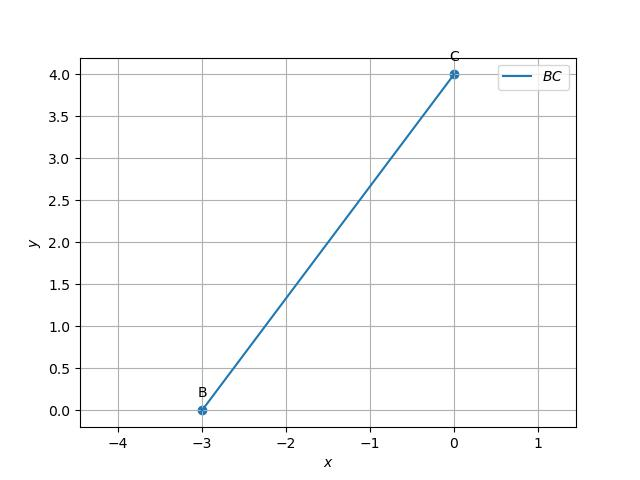
\includegraphics [width=\columnwidth] {/sdcard/hima/geometry/figs/cust.jpg}
\caption{ The line $\vec{BC}$ plotted using python}
\label{fig: linebc}
\end{figure}



The normal equation for the side $CA$ is
\begin{align}
\vec{n}^{\top}\myvec{\vec{x}-\vec{C}}&=0\\
\implies
\vec{n}^{\top}\vec{x}&=\vec{n}^{\top}\vec{C}
\end{align}
Now our task is to find the $\vec{n}$ so that we can find $\vec{n}^{\top}$.
As given in the question 
\begin{align}
  \vec{n} &= \myvec{0 & 1\\
  -1 & 0}\vec{m}
\end{align}
Here $\vec{m} = \vec{A}- \vec{C}$ for side $\vec{CA}$
\begin{align}
\implies
\vec{m}&=\myvec{1\\3} - \myvec{0\\4}\\
&=\myvec{1\\-1}
\end{align}
Now as we have obtained vector $\vec{m}$.
we can use this to obtain vector $\vec{n}$
\begin{align}
\vec{n} &= \myvec{0 & 1\\
  -1 & 0}\myvec{1\\-1}
 = \myvec{-1\\1}
\end{align}
The transpose of $\vec{n}$ is
\begin{align}
  \vec{n}^{\top}&=\myvec{-1 & 1}
\end{align}
Hence the normal equation of side $CA$ is 
\begin{align}
    \myvec{-1 & 1}\vec{x}&=\myvec{-1 & 1}\myvec{0\\4}\\
    \implies
    \myvec{12 & 1}\vec{x}& = -4
\end{align}
\begin{figure}[H]
	\centering
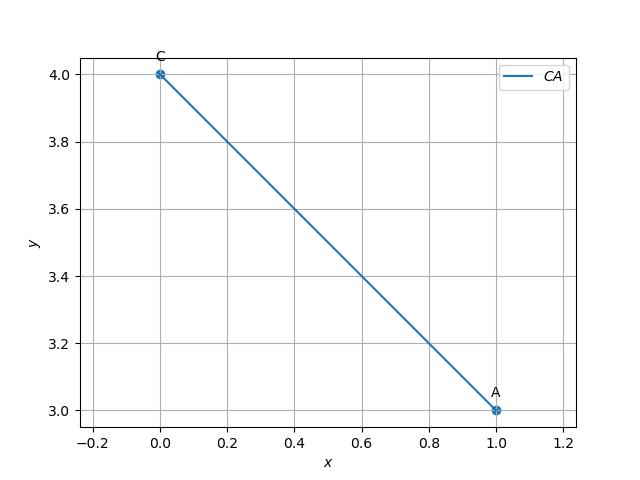
\includegraphics [width=\columnwidth] {/sdcard/hima/geometry/figs/hert.jpg}
\caption{ The line $\vec{CA}$ plotted using python}
\label{fig: lineca}
\end{figure}


\item The area of $\triangle ABC$ is defined as
		\begin{align}
			\frac{1}{2}\norm{{\brak{\vec{A}-\vec{B}}\times {\vec{A}-\vec{C}}}}
		\end{align}
		where
		\begin{align}
			\vec{A}\times\vec{B} \triangleq \mydet{1 & -3 \\3 & 0}
		\end{align}
Question 1.1.6:Find the area of $\triangle$ ABC.\\
\solution
Given,
\begin{align}
\vec{A} = \myvec{1\\3};
\vec{B} = \myvec{-3\\0};
\vec{C} = \myvec{0\\4}\\
\vec{A}-\vec{B}=\myvec{1\\3}-\myvec{-3\\0}&=\myvec{4\\3}\\
\vec{A}-\vec{C}=\myvec{1\\3}-\myvec{0\\4}&=\myvec{1\\-1}\\
\therefore(\vec{A}-\vec{B})\times(\vec{A}-\vec{C}) &=\mydet{4 & 1\\3 & -1}\\
	&=(4)\times (-1)- 3\times -1\\&= -4-3\\&=-7\\
\implies\frac{1}{2}\norm{(\vec{A}-\vec{B})\times(\vec{A}-\vec{C})}&=\frac{-7}{2}= -3.5
\end{align}


\item
Question 1.1.7:Find the angles $\vec{A},\vec{B},\vec{C}$, given that 
\begin{align}
	\cos{A} \triangleq \frac{(\vec{B}-\vec{A})\top(\vec{C}-\vec{A})}{\norm{\vec{B}-\vec{A}}\norm{\vec{C}-\vec{A}}}
\end{align}
\solution 
\\
From the given values of $\vec{A},\vec{B},\vec{C}$,\\
\begin{enumerate}

\item Finding the value of angle A
\begin{align}
	\vec{B}-\vec{A} &=\myvec{-4\\-3}
\end{align}
and 
\begin{align}
	\vec{C}-\vec{A}&= \myvec{-1\\1}
\end{align}
also calculating the values of norms
\begin{align}
	\norm{\vec{B}-\vec{A}} &= \sqrt{25} &= 5\\
	\norm{\vec{C}-\vec{A}} &= \sqrt{2}
\end{align}
and by doing matrix multiplication we get,
\begin{align}
\begin{split}
	(\vec{B}-\vec{A})^{\top}(\vec{C}-\vec{A})&=\myvec{-4 & -3}\myvec{-1\\ 1}\\
	&= 1
\end{split}
\end{align}
so 
\begin{align}
	\cos{A}&= \frac{-8}{5 \sqrt{2}}\\
	\implies A&=\cos^{-1}{\frac{-8}{5\sqrt{2}}}
\end{align}




\item Finding the value of angle B
\begin{align}
	\vec{C}-\vec{B} &=\myvec{3\\ -4}
\end{align}
and 
\begin{align}
	\vec{A}-\vec{B}&= \myvec{4\\3}
\end{align}
also calculating the values of norms
\begin{align}
	\norm{\vec{C}-\vec{B}} &= \sqrt{25} =5\\
	\norm{\vec{A}-\vec{B}} &= \sqrt{25} =5
\end{align}
and by doing matrix multiplication we get,
\begin{align}
\begin{split}
	(\vec{C}-\vec{B})^{\top}(\vec{A}-\vec{B})&=\myvec{ 3& -4}\myvec{3\\-4}\\
	&= 25
\end{split}
\end{align}
so 
\begin{align}
	\cos{B}&= \frac{25}{\sqrt{25} \sqrt{25}}\\
	&= \frac{25}{\ {25}} = 1\\
	\implies B&=\cos^{1} = 0
\end{align}



\item Finding the value of angle C
\begin{align}
	\vec{A}-\vec{C} &=\myvec{1\\-1}
\end{align}
and 
\begin{align}
	\vec{B}-\vec{C}&= \myvec{-3\\-4}
\end{align}
also calculating the values of norms
\begin{align}
	\norm{\vec{A}-\vec{C}} &= \sqrt{2}\\
	\norm{\vec{B}-\vec{C}} &= \sqrt{25} =5
\end{align}
and by doing matrix multiplication we get,
\begin{align}
\begin{split}
	(\vec{A}-\vec{C})^{\top}(\vec{B}-\vec{C})&=\myvec{1&-1}\myvec{-3\\-4}\\
	&=1
\end{split}
\end{align}
so 
\begin{align}
\cos{C}&= \frac{1}{ 5 \sqrt{2}}\\
	\implies C&=\cos^{-1}{\frac{1}{5 \sqrt{2}}}
\end{align}

\end{enumerate}


\end{enumerate}









%\section{Median}
%\input{subsec/median}
%\section{Altitude}
%\section{Perpendicular Bisector}
%\section{Angle Bisector}

\end{document}
